% !TEX root = ../main.tex

%%% ============================================================
\section{Phương pháp HSGE}
%%% ============================================================

\subsection{Giải pháp HSGE: đóng góp chính}
\begin{frame}{Giải pháp HSGE và các đóng góp chính}
  \begin{columns}[t]

    \begin{column}{0.49\textwidth}
      \uncover<1->{
        \head{Đóng góp Khoa học}
        \begin{itemize}\ilist
          \item \textbf{Đồ thị hai tầng}: State Graph $\leftrightarrow$ Operator Graph. \kw{[T2]}
          \item \textbf{Quy nạp \& ghép chuỗi}: skill $\rightarrow$ operator $\rightarrow$ task đa bước. \kw{[T4]}
          \item \textbf{Kiểm định trực tuyến}: loại dương tính giả ngay lúc chạy. \kw{[T3]}
        \end{itemize}
      }
    \end{column}
    \hfill
    \begin{column}{0.47\textwidth}
      \uncover<2->{
        \head{Đóng góp Thực tiễn}
        \begin{itemize}\ilist
          \item \textbf{Dataset SFT}: \kw{9.007 mẫu} / 4 website, \kw{0 nhãn con người}. \kw{[T1]}
          \item \textbf{HSGE-9B}: đạt \kw{24,6\%} (vượt GPT-4o-mini).
          \item \textbf{Kinh tế}: \kw{\$0,0308}/trajectory (\kw{rẻ hơn 3,3$\times$}).
        \end{itemize}
      }
    \end{column}
  \end{columns}

  \gap
  \uncover<2->{
    \begin{beamercolorbox}[wd=\textwidth,sep=2.5pt,leftskip=6pt,rightskip=6pt,rounded=true]{block body}
      \footnotesize Phần còn lại của mục này: bốn thách thức \textbf{T1--T4} được giải quyết trong một quy trình khép kín.
    \end{beamercolorbox}
  }
\end{frame}

\subsection{Tổng quan kiến trúc pipeline}
\begin{frame}{Tổng quan pipeline HSGE}
  \begin{center}
    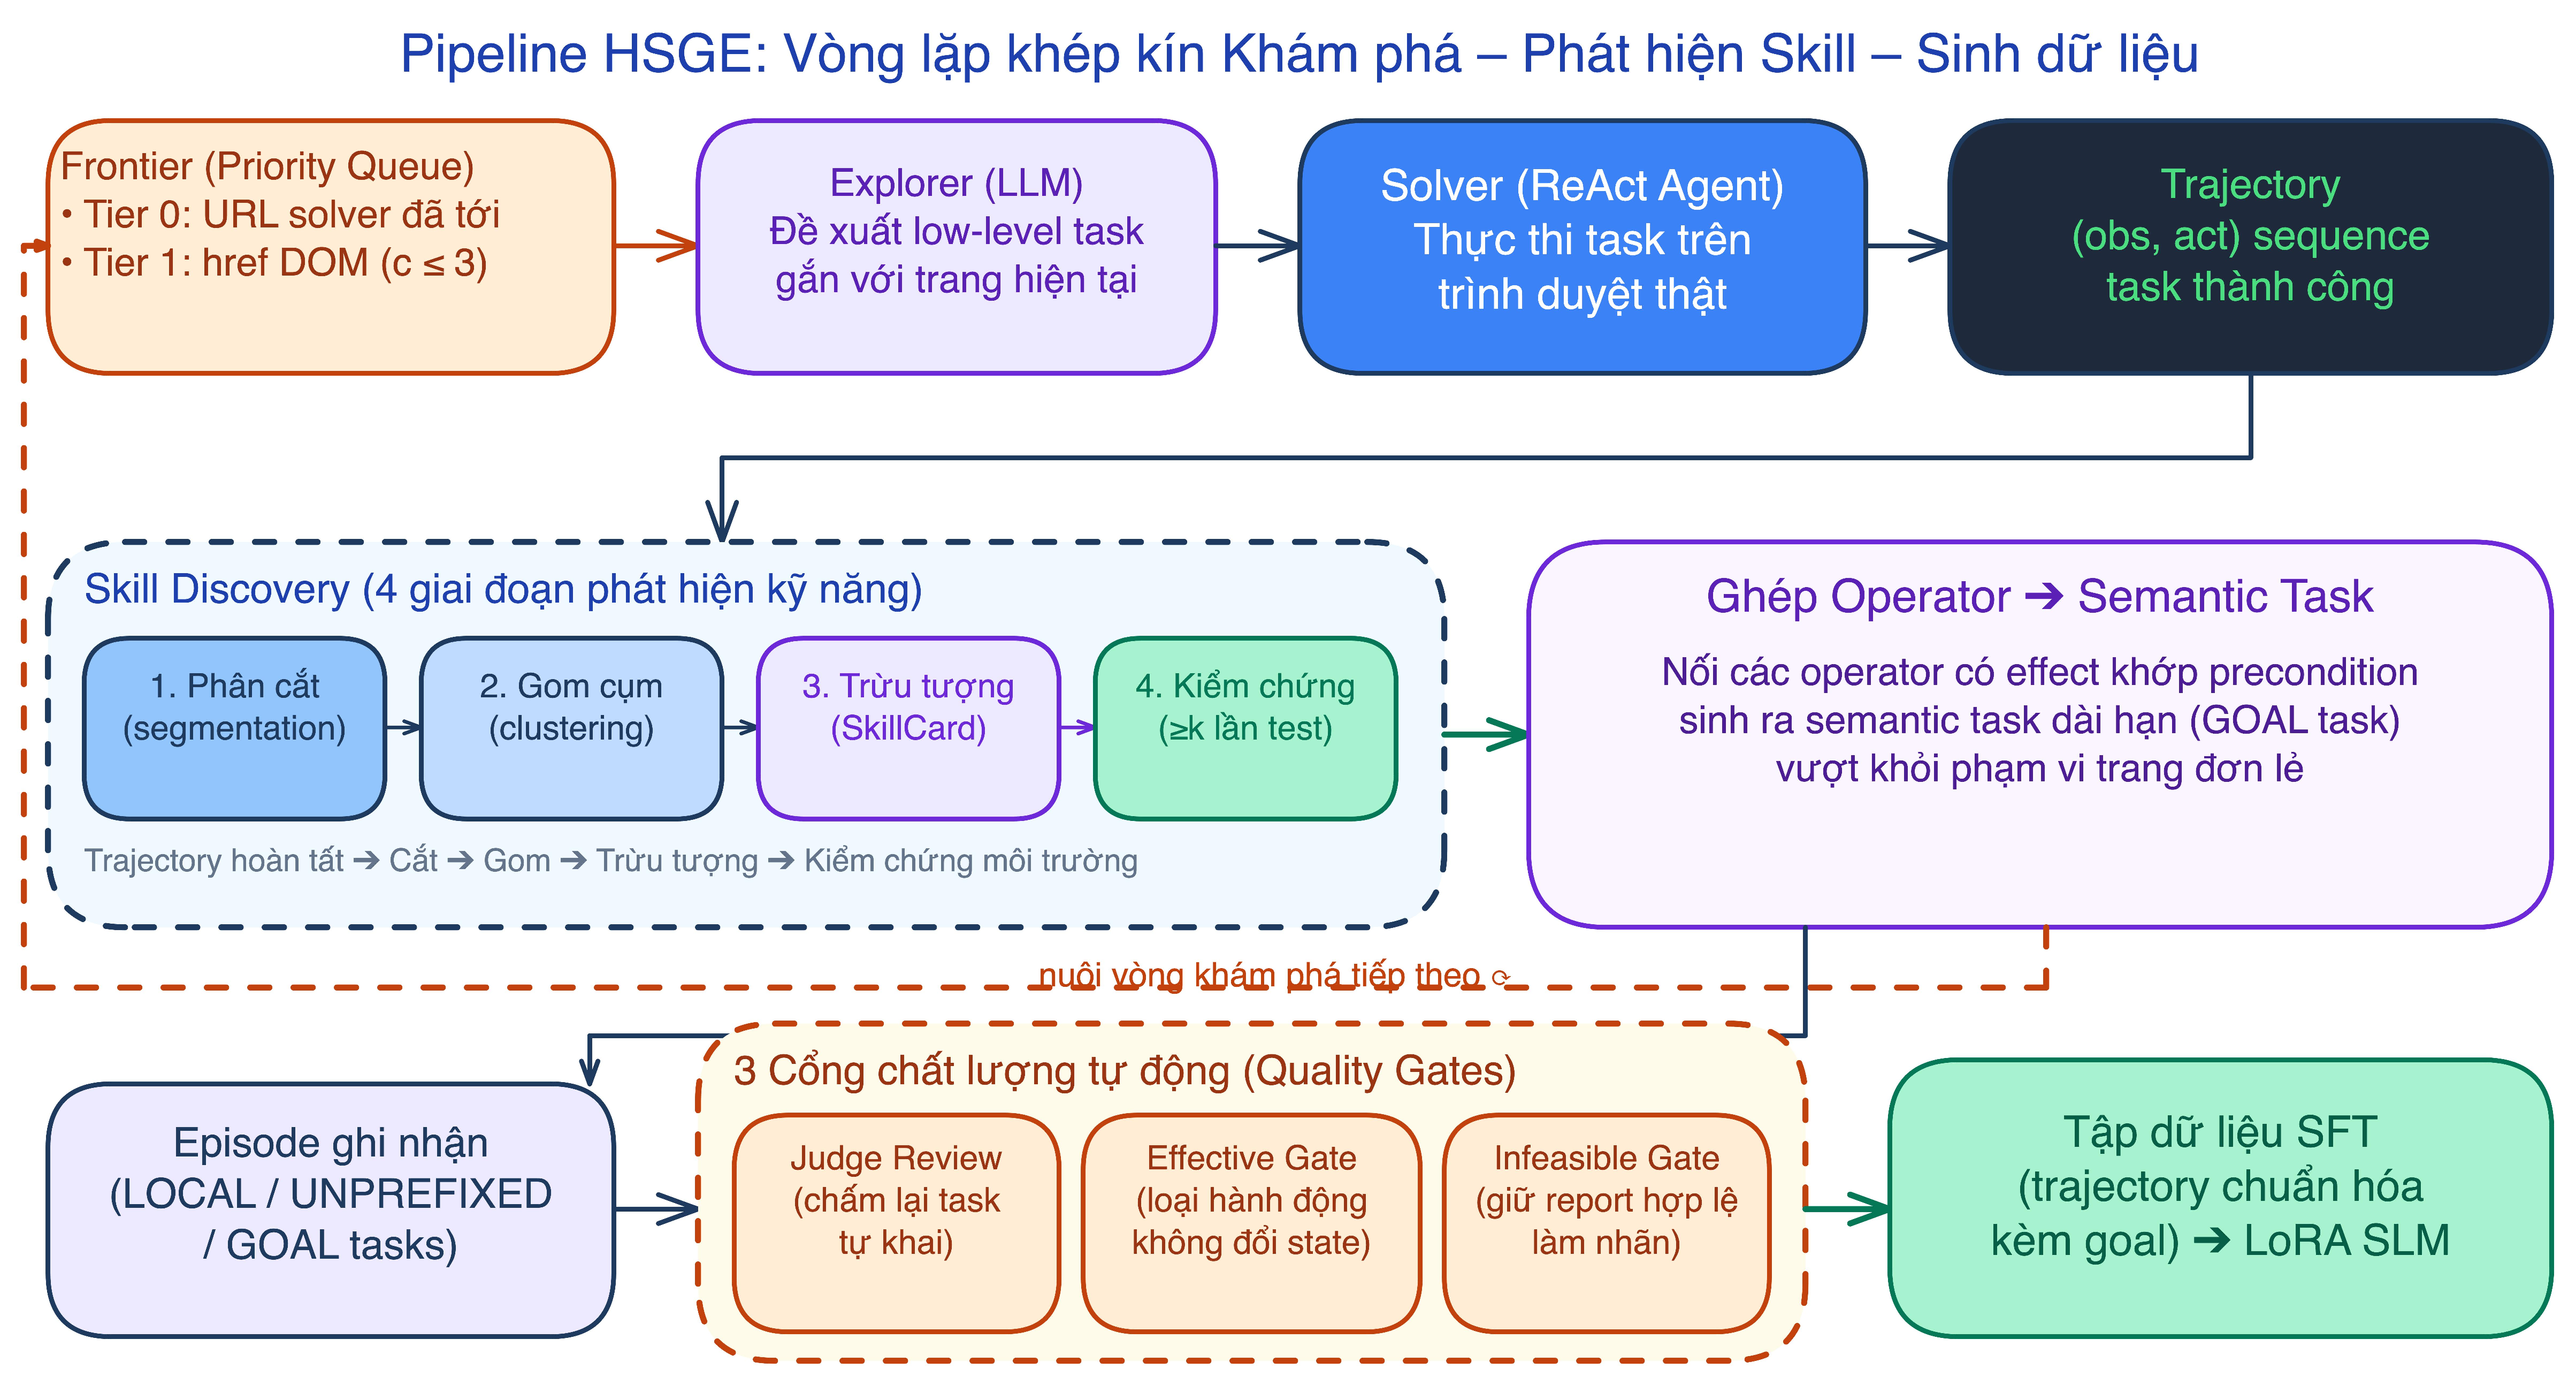
\includegraphics[width=\linewidth,height=0.86\textheight,keepaspectratio]{fig_pipeline.pdf}
  \end{center}
  \vspace{-0.1cm}
  \begin{center}
    \footnotesize
    \kw{Frontier} $\xrightarrow{\text{duyệt}}$ \textbf{Explorer/Solver} $\xrightarrow{\text{quy nạp}}$ \kw{Skill/Operator} $\xrightarrow{\text{ghép chuỗi}}$ \textbf{Semantic Task} $\xrightarrow{\text{lọc online}}$ \kw{Dataset SFT}
  \end{center}
\end{frame}

\subsection{Khám phá tự hành}
\begin{frame}{Khám phá tự hành: một vòng lặp trên một trang}
  \begin{columns}[onlytextwidth,t]
    \begin{column}{0.585\textwidth}
      \uncover<1->{
        \begin{hblock}{Năm bước của một vòng lặp}{\bhH}
          \begin{enumerate}\ilist
            \item \textbf{Lấy trang}: pop URL khỏi \kw{Frontier}, mở browser, đọc \kw{AXTree}.
            \item \textbf{Sinh task}: Explorer đề xuất $\le 9$ task \kw{từ chính trang đó} (INFO / NAV / MOD).
            \item \textbf{Giải task}: Solver chạy \kw{ReAct}, $15$ bước ($25$ nếu đa bước).
            \item \textbf{Kiểm định}: Judge soi trang đích; task đạt \kw{giải lại từ trang gốc}.
            \item \textbf{Mở rộng Frontier}: URL đã ghé $+$ liên kết trên trang.
          \end{enumerate}
        \end{hblock}
      }
    \end{column}

    \hfill
    \begin{column}{0.385\textwidth}
      \uncover<2->{
        \begin{hblock}{Bốn chốt chặn thoái hóa}{\bhH}
          \begin{itemize}\ilist
            \item \textbf{Node trùng}: băm nội dung AXTree $\rightarrow$ loại \kw{71/455} node.
            \item \textbf{Lặp thao tác}: dừng cứng khi cùng đích mà trang không đổi.
            \item \textbf{Bão hòa}: $\le 3$ node mỗi \kw{khuôn dạng} URL.
            \item \textbf{Task trùng}: nhớ task đã đề xuất, bỏ các bản gần trùng.
          \end{itemize}
        \end{hblock}
      }
    \end{column}
  \end{columns}

  \gap
  \uncover<3->{
    \begin{beamercolorbox}[wd=\textwidth,sep=2.5pt,leftskip=6pt,rightskip=6pt,rounded=true]{block body}
      \footnotesize \kw{Kết quả trên 4 website}: \kw{455} trang được khám phá, \kw{3.981} lượt thử, \kw{2.117} trajectory hợp lệ (\kw{53,2\%}).
    \end{beamercolorbox}
  }
\end{frame}

\subsection{Phát hiện Skill \& Quy nạp Operator}
\begin{frame}{Phát hiện skill và quy nạp operator}
  \begin{columns}[c]
    \begin{column}{0.48\textwidth}
      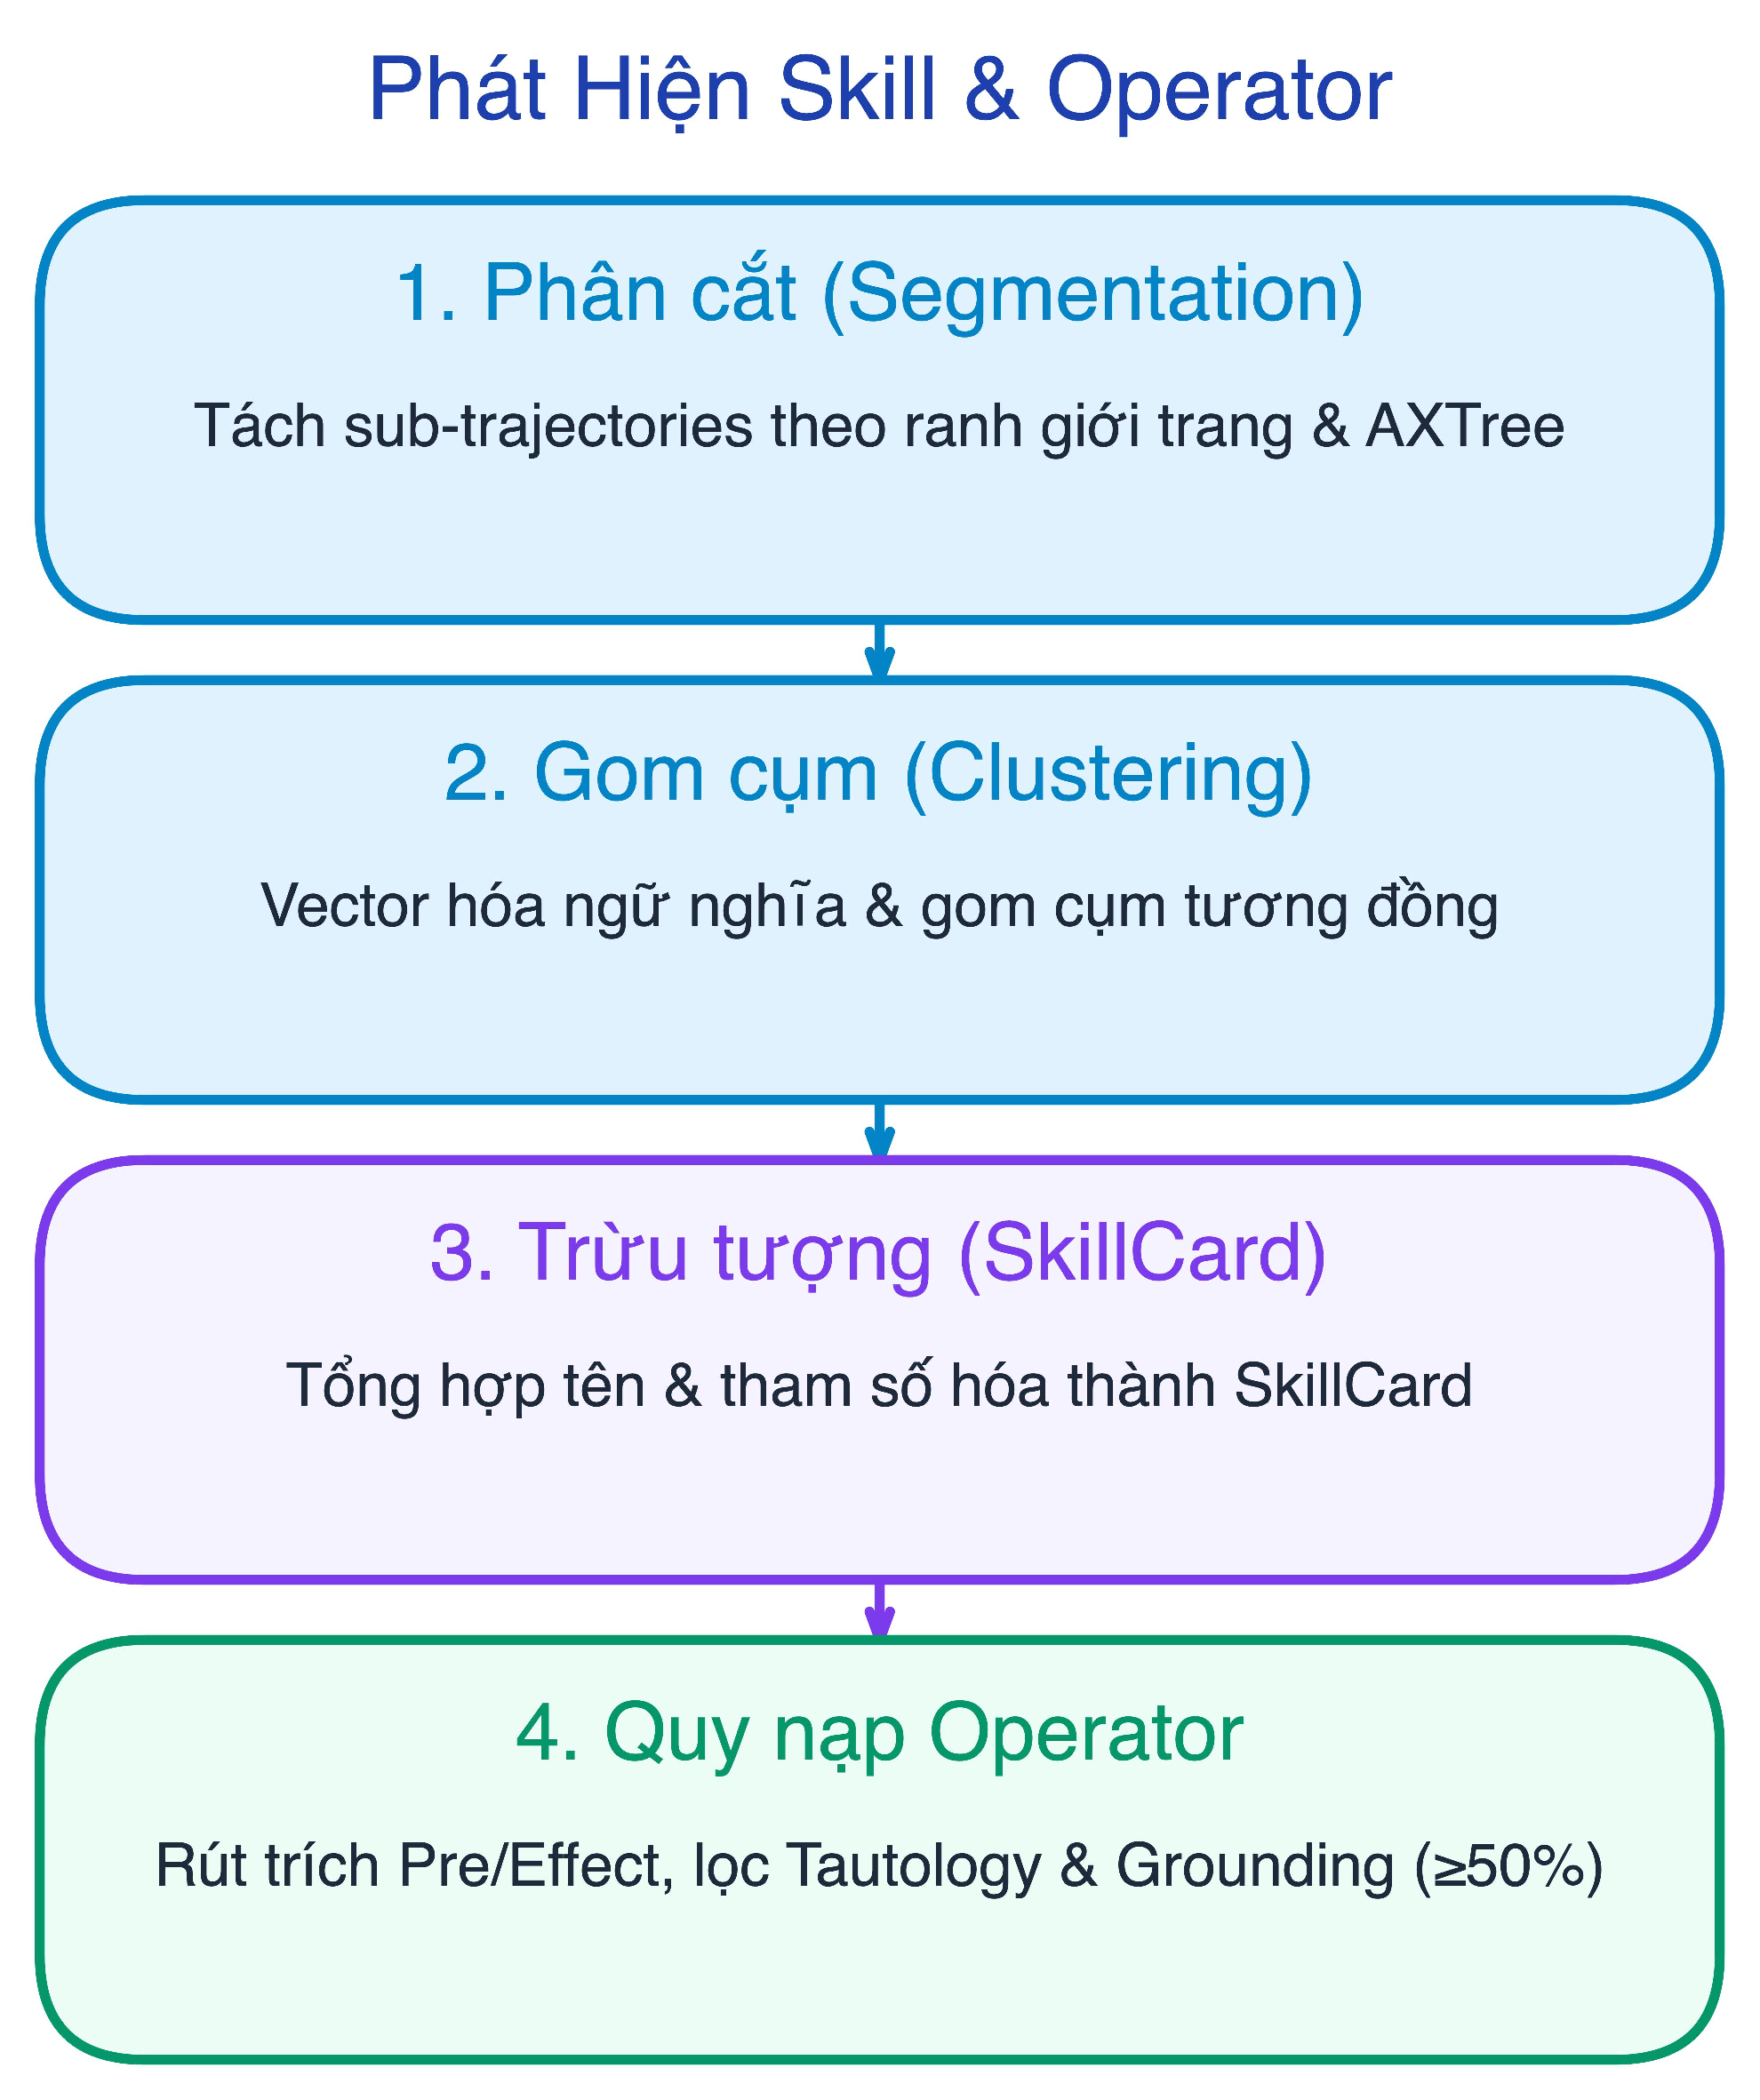
\includegraphics[width=\linewidth,height=0.85\textheight,keepaspectratio]{fig_discovery.pdf}
    \end{column}
    \hfill
    \begin{column}{0.50\textwidth}
      \uncover<1->{
        \head{4 bước phát hiện skill}
        \begin{enumerate}\ilist
          \item \textbf{Phân cắt}: đổi URL \& tụt tương đồng AXTree.
          \item \textbf{Gom cụm}: phi tham số (ngưỡng cosine).
          \item \textbf{Trừu tượng hóa}: \textit{SkillCard} tham số hóa.
          \item \textbf{Kiểm chứng}: chạy lại trong ngữ cảnh mới.
        \end{enumerate}
      }

      \vspace{0.1cm}
      \uncover<2->{
        \begin{block}{Quy nạp Operator \& Cổng chặn}
          \begin{itemize}\ilist
            \item \textbf{Chống trùng}: loại effect lặp lại precondition.
            \item \textbf{Grounding}: gỡ effect sai trên $\ge 50\%$ thành viên.
            \item $\Rightarrow$ \kw{146 skill} $\rightarrow$ \kw{57 operator}.
          \end{itemize}
        \end{block}
      }
    \end{column}
  \end{columns}
\end{frame}

\subsection{Sinh Semantic Task từ chuỗi Operator}
\begin{frame}{Sinh semantic task: ghép chuỗi operator}
  \begin{center}
    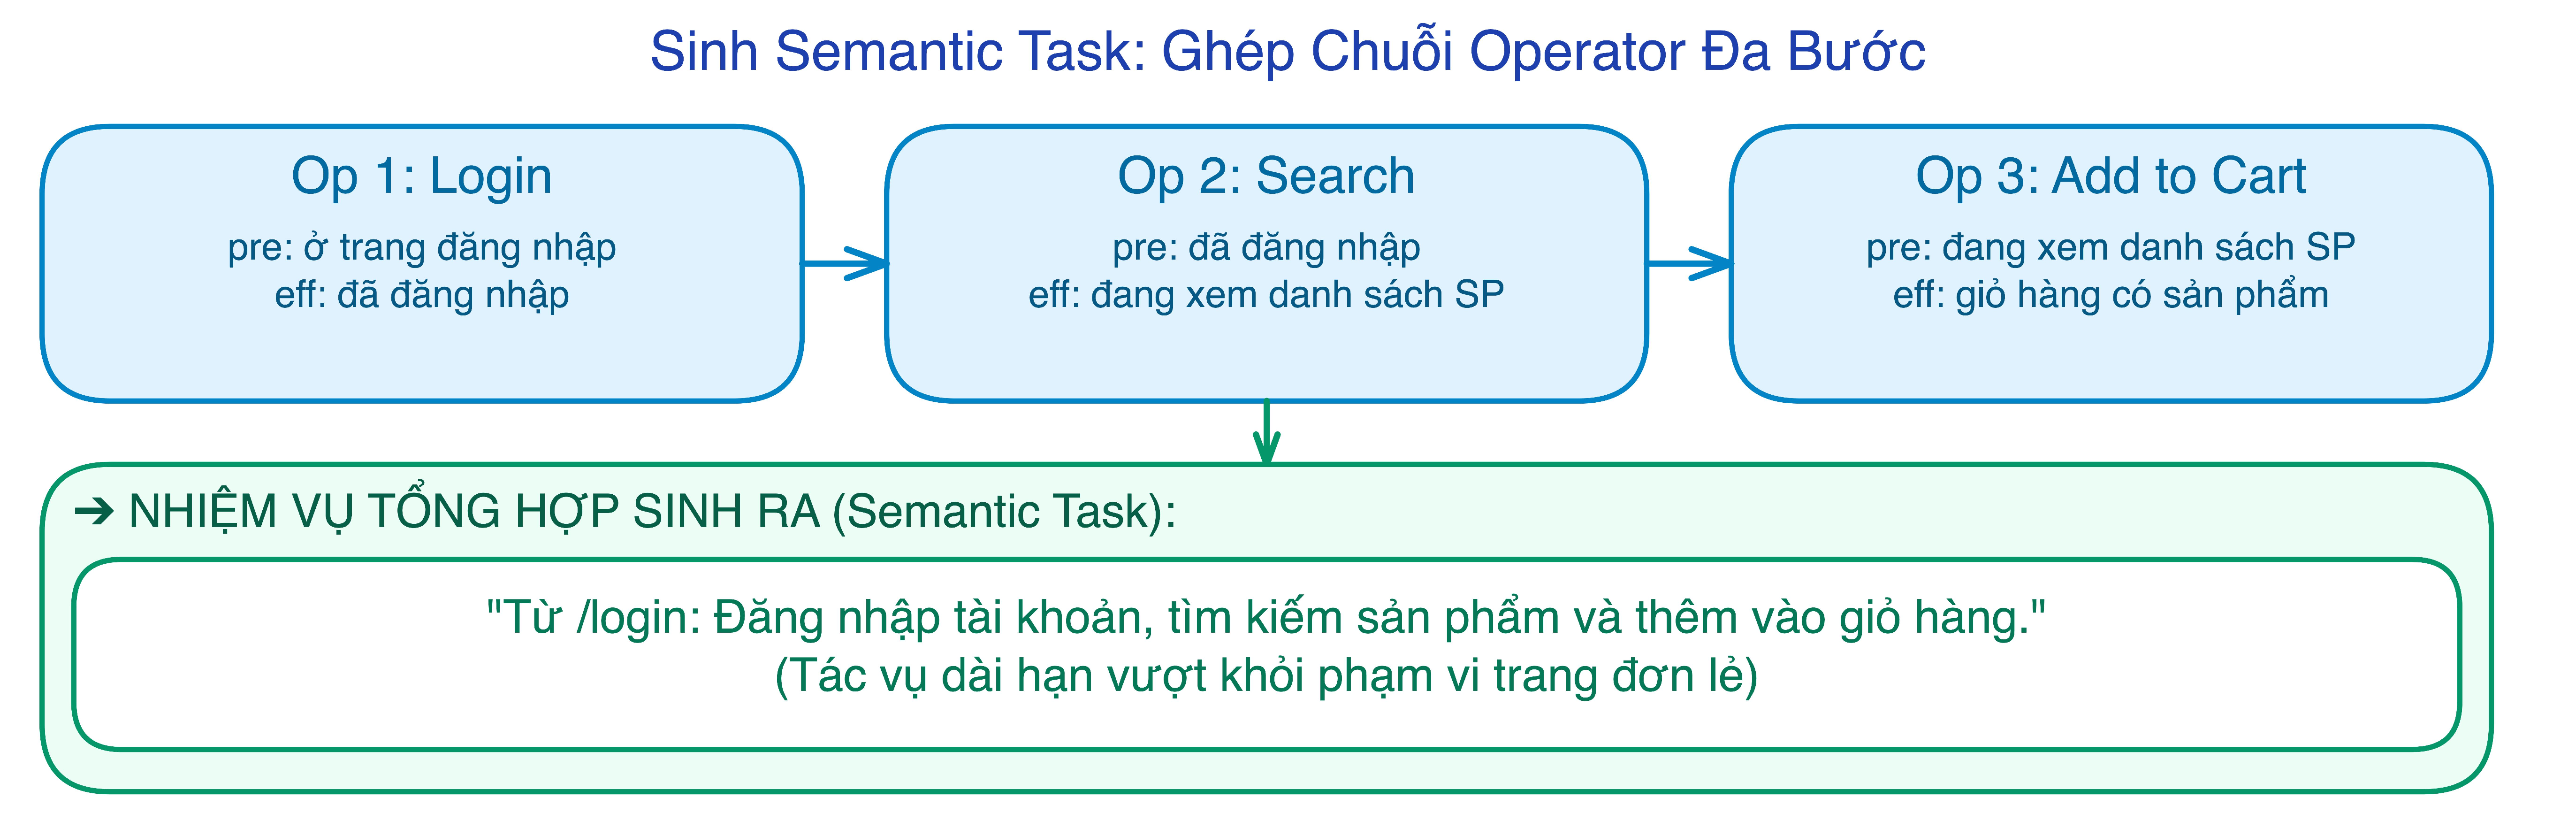
\includegraphics[width=0.95\linewidth,height=0.46\textheight,keepaspectratio]{fig_semantic.pdf}
  \end{center}
  \vspace{-0.15cm}
  \begin{columns}[t]
    \begin{column}{0.48\textwidth}
      \uncover<1->{
        \head{Hai cơ chế sinh tác vụ nhiều bước}
        \begin{itemize}\ilist
          \item \textbf{Bottom-up}: DFS đồ thị operator; chuỗi $\ge 2$ $\rightarrow$ task dài.
          \item \textbf{Top-down}: seed từ chức năng tổng quan website.
        \end{itemize}
      }
    \end{column}
    \hfill
    \begin{column}{0.48\textwidth}
      \uncover<2->{
        \begin{alertblock}{Kết quả thực thi}
          \footnotesize Sinh \kw{142 task} (130 seed + 12 chuỗi) $\rightarrow$ \kw{71 task thành công}.
        \end{alertblock}
      }
    \end{column}
  \end{columns}
\end{frame}

\subsection{Kiểm định trực tuyến \& Đóng gói SFT}
\begin{frame}{Kiểm định trực tuyến và đóng gói SFT}
  \begin{columns}[c]
    \begin{column}{0.46\textwidth}
      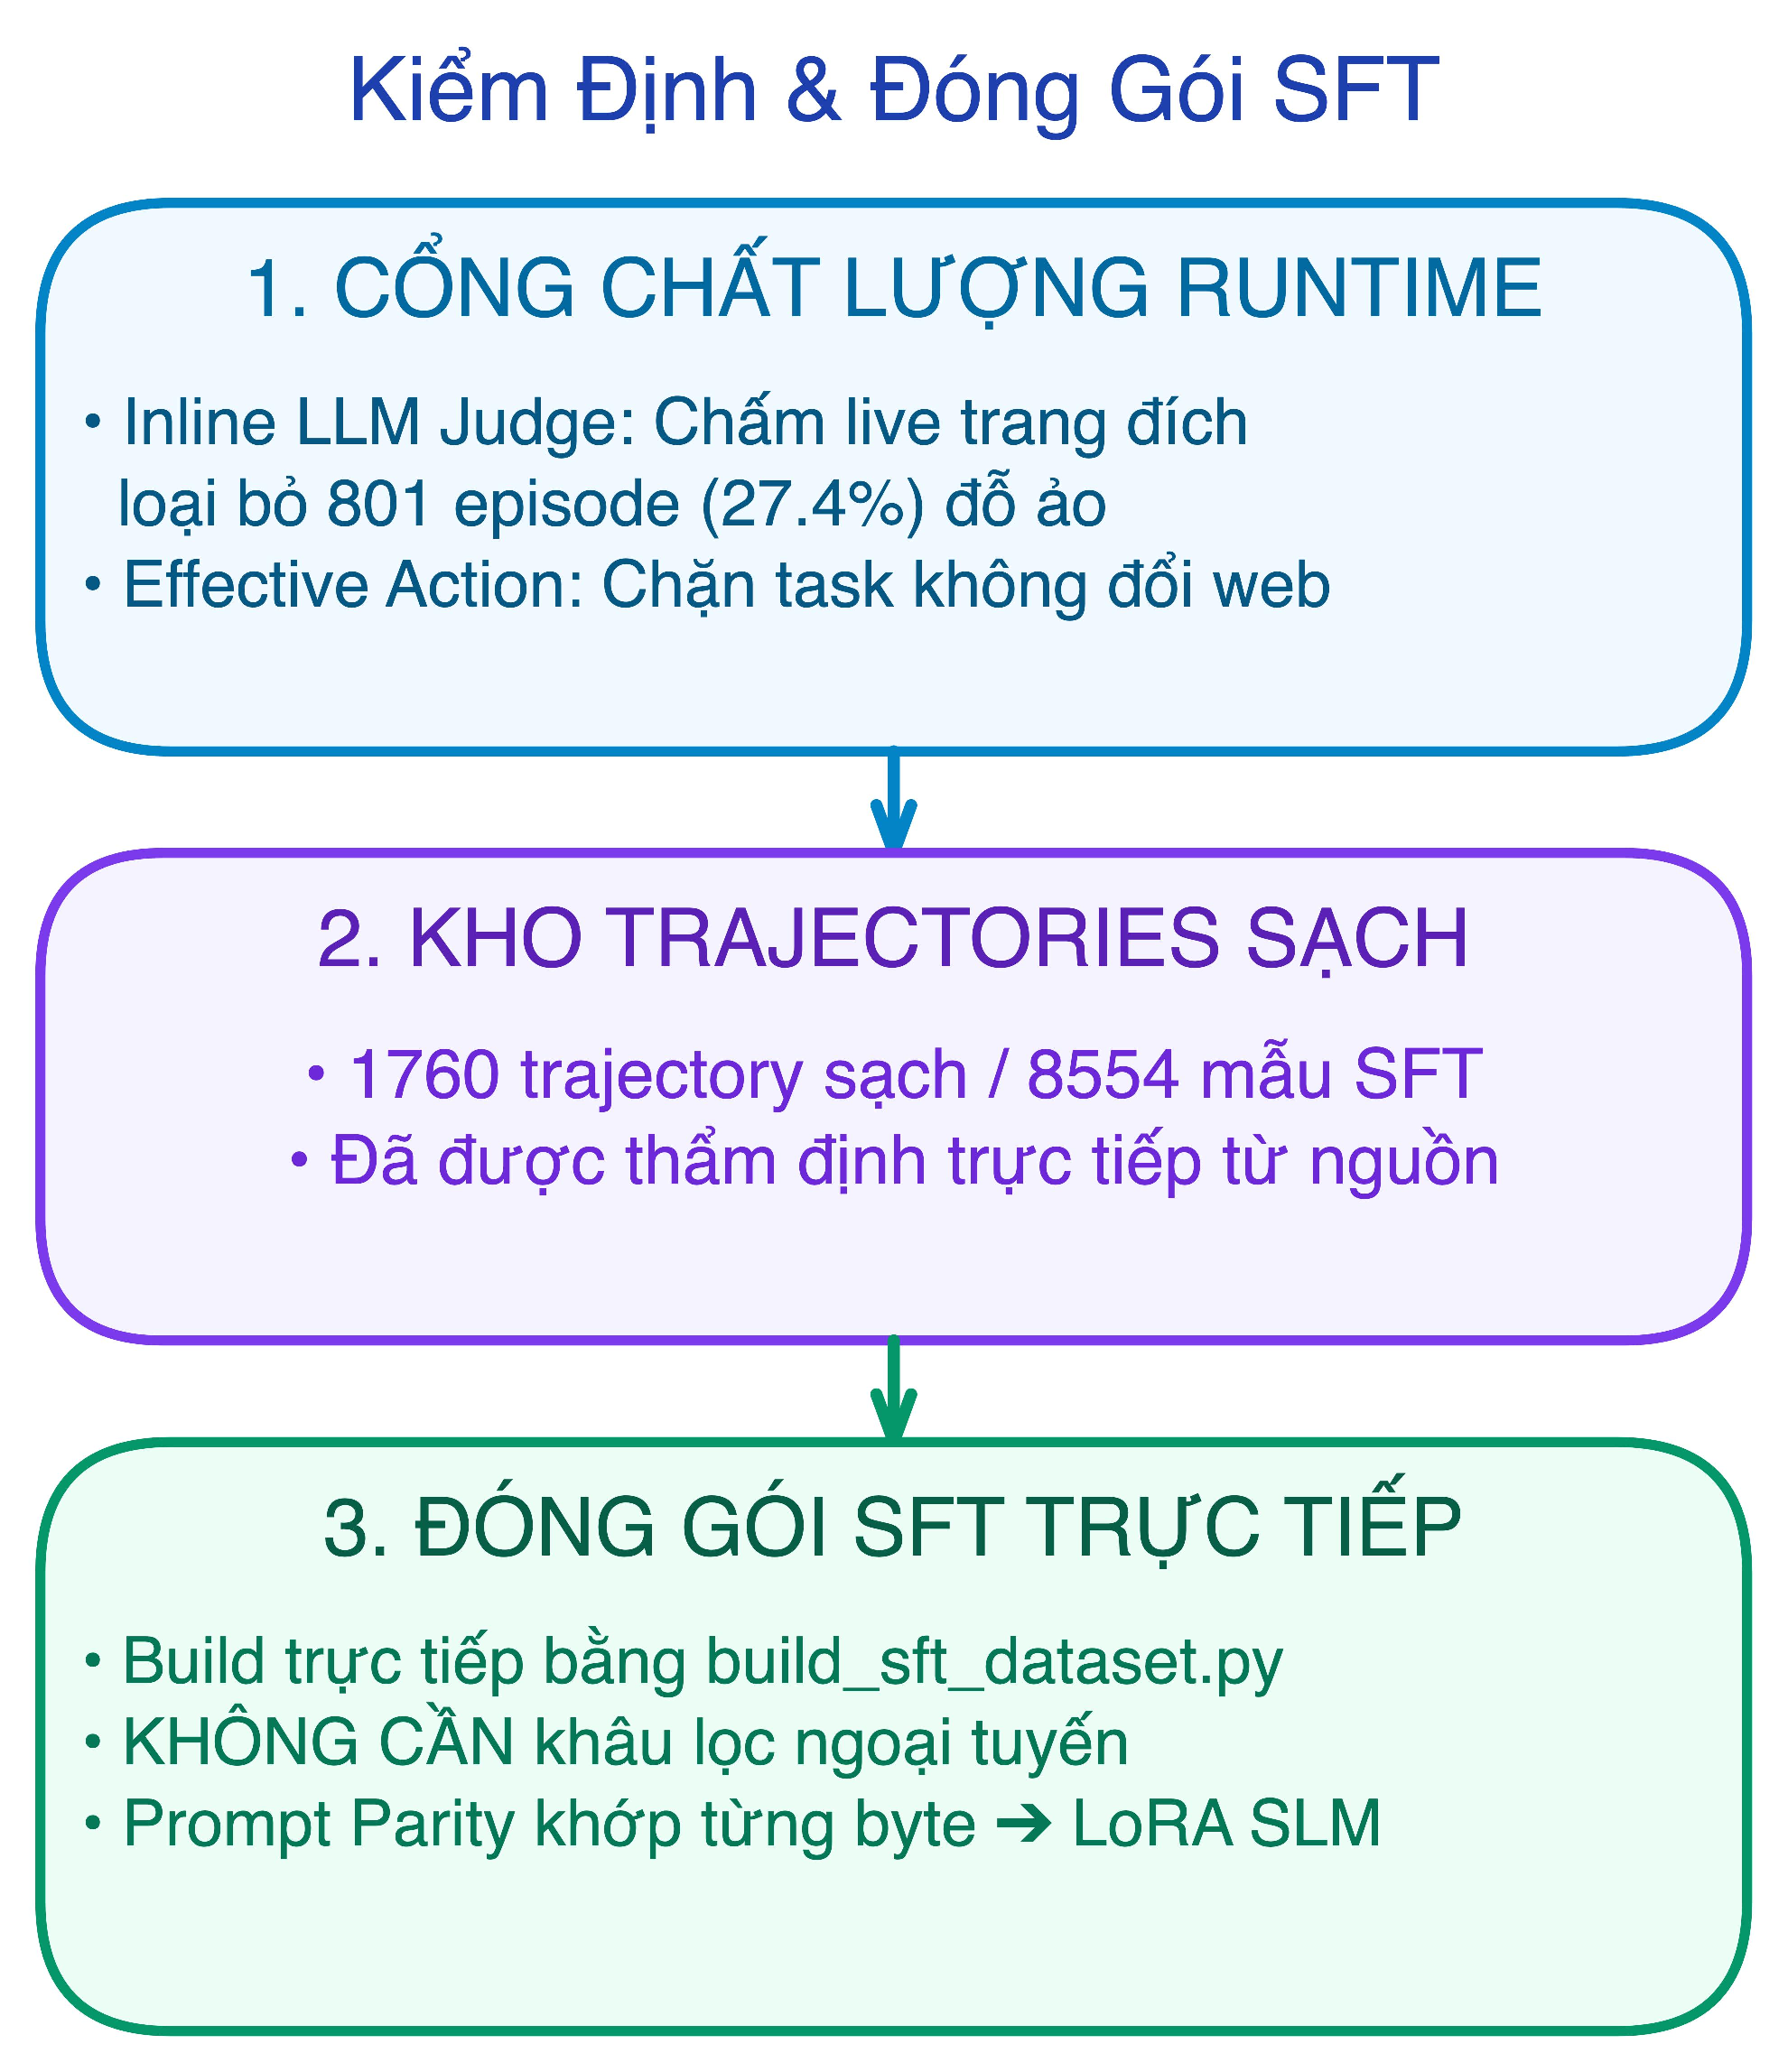
\includegraphics[width=\linewidth,height=0.85\textheight,keepaspectratio]{fig_curation.pdf}
    \end{column}
    \hfill
    \begin{column}{0.52\textwidth}
      \uncover<1->{
        \head{Kiểm soát chất lượng (Online Gates)}
        \begin{itemize}\ilist
          \item \textbf{Online LLM Judge}: chấm lại trang đích $\rightarrow$ loại \kw{801 episode (27,4\%)}.
          \item \textbf{Effective Action}: loại task không đổi trạng thái $\rightarrow$ \kw{1760 trajectory sạch}.
        \end{itemize}
      }

      \vspace{0.08cm}
      \uncover<2->{
        \begin{block}{Đóng gói SFT \& Prompt Parity}
          \begin{itemize}\ilist
            \item \textbf{Build trực tiếp}: sạch từ nguồn, không lọc ngoại tuyến.
            \item \textbf{Prompt Parity}: khớp từng byte train / suy luận.
            \item $\Rightarrow$ \kw{8554 train / 453 val} (0 trùng lặp).
          \end{itemize}
        \end{block}
      }
    \end{column}
  \end{columns}
\end{frame}

